\subsubsection{Module 2: Tương tác Xã hội}
Module này tập trung vào các tính năng kết nối cộng đồng, chia sẻ nội dung và tương tác giữa người mua và người bán, tạo tiền đề cho các hoạt động thương mại.

\begin{figure}[H]
\centering
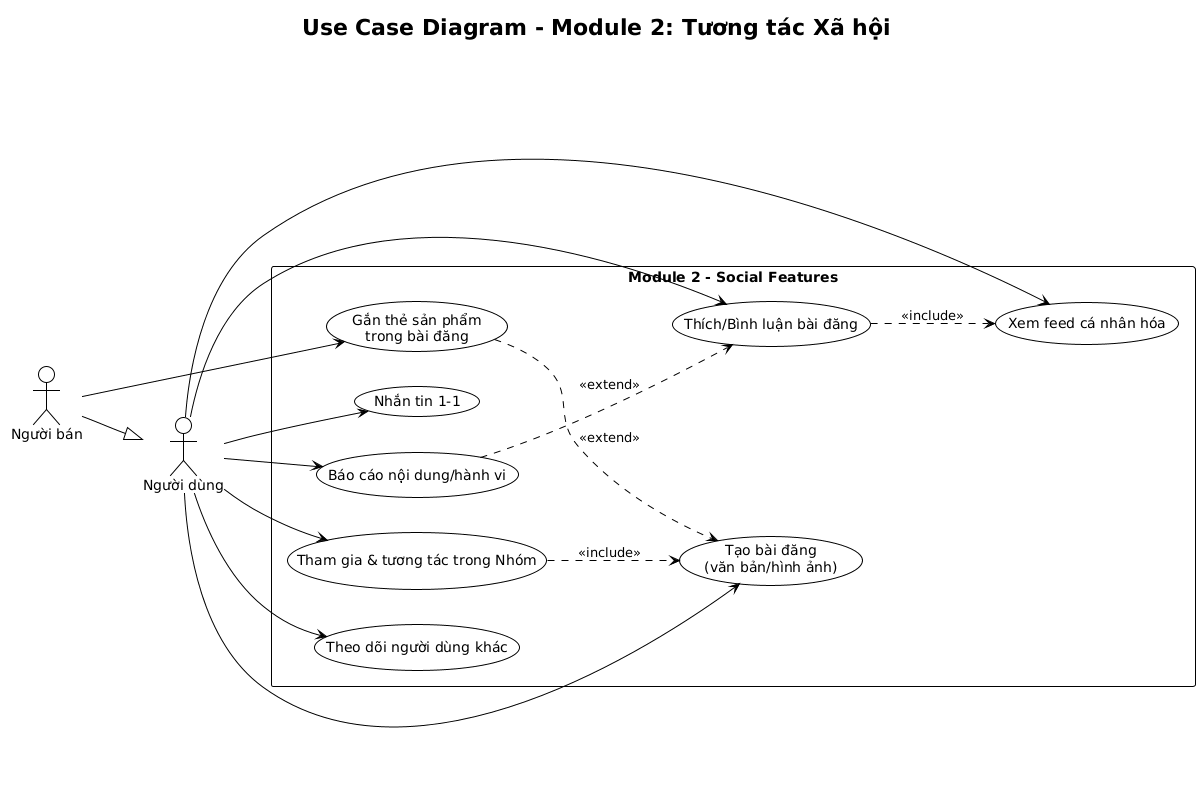
\includegraphics[width=\textwidth]{Images/Usecases/UC-M2-Social.png}
\caption{Sơ đồ Use Case cho Module 2: Tương tác Xã hội}
\label{fig:usecase-module2}
\end{figure}

% Cấu hình giãn dòng
\renewcommand{\arraystretch}{1.3}

% =====================================================
% UC2.1: XEM BẢNG TIN
% =====================================================
\begin{table}[H]
\centering
\begin{tabularx}{\textwidth}{|l|X|}
\hline
\textbf{Tên Use Case} & \textbf{UC2.1: Xem bảng tin (Feed) cá nhân hóa} \\ \hline
\textbf{Tác nhân} & Người dùng \\ \hline
\textbf{Mô tả} & Hiển thị một Bảng tin (Feed) được cá nhân hóa cho người dùng, ưu tiên hiển thị các bài đăng từ những người họ theo dõi và các bài viết có tương tác cao. \\ \hline
\textbf{Kích hoạt} & Người dùng truy cập vào trang chủ sau khi đăng nhập. \\ \hline
\textbf{Điều kiện tiên quyết} & Người dùng đã đăng nhập vào hệ thống. \\ \hline
\textbf{Điều kiện sau} & Người dùng xem được danh sách các bài đăng mới nhất và phù hợp nhất. \\ \hline
\textbf{Luồng sự kiện chính} & 
\begin{enumerate}
    \item Người dùng đăng nhập thành công và được chuyển hướng đến trang chủ.
    \item Hệ thống truy vấn cơ sở dữ liệu để lấy danh sách bài đăng từ những người dùng mà họ đang theo dõi.
    \item Hệ thống cũng lấy các bài đăng có mức độ tương tác cao hoặc được gợi ý.
    \item Hệ thống sắp xếp các bài đăng theo thuật toán (ví dụ: mới nhất, tương tác cao nhất) và hiển thị cho người dùng.
    \item Khi người dùng cuộn trang, hệ thống sẽ tải thêm các bài đăng cũ hơn (infinite scroll).
\end{enumerate} \\ \hline
\textbf{Ngoại lệ} & E1: Lỗi tải dữ liệu $\rightarrow$ Hệ thống hiển thị thông báo lỗi và nút ``Thử lại''. \\ \hline
\textbf{Ghi chú} & Thuật toán sắp xếp feed có thể được cải tiến trong tương lai để tăng tính cá nhân hóa. \\ \hline
\end{tabularx}
\caption{Đặc tả Use Case Xem Bảng tin}
\end{table}

% =====================================================
% UC2.2: TẠO BÀI ĐĂNG
% =====================================================
\begin{table}[H]
\centering
\begin{tabularx}{\textwidth}{|l|X|}
\hline
\textbf{Tên Use Case} & \textbf{UC2.2: Tạo bài đăng (văn bản, hình ảnh)} \\ \hline
\textbf{Tác nhân} & Người dùng \\ \hline
\textbf{Mô tả} & Cho phép người dùng tạo và chia sẻ các bài đăng với nội dung văn bản và hình ảnh lên trang cá nhân của họ và Bảng tin của những người theo dõi. \\ \hline
\textbf{Kích hoạt} & Người dùng nhấn vào nút ``Tạo bài đăng'' trên giao diện. \\ \hline
\textbf{Điều kiện tiên quyết} & Người dùng đã đăng nhập vào hệ thống. \\ \hline
\textbf{Điều kiện sau} & 
\begin{itemize}
    \item Một bài đăng mới được tạo và lưu vào cơ sở dữ liệu.
    \item Bài đăng mới xuất hiện trên trang cá nhân của người dùng và Bảng tin của những người theo dõi.
\end{itemize} \\ \hline
\textbf{Luồng sự kiện chính} & 
\begin{enumerate}
    \item Người dùng nhấn vào ô tạo bài đăng.
    \item Người dùng nhập nội dung văn bản.
    \item Người dùng tùy chọn tải lên một hoặc nhiều hình ảnh.
    \item Người dùng nhấn nút ``Đăng''.
    \item Hệ thống kiểm tra tính hợp lệ của nội dung.
    \item Hệ thống lưu bài đăng vào cơ sở dữ liệu.
    \item Hệ thống hiển thị bài đăng mới ngay trên giao diện của người dùng.
\end{enumerate} \\ \hline
\textbf{Luồng thay thế} & A1: Người dùng hủy bỏ việc tạo bài đăng, nội dung nháp sẽ bị xóa. \\ \hline
\textbf{Ngoại lệ} & 
\begin{itemize}
    \item E1: Lỗi tải lên hình ảnh (kích thước quá lớn, định dạng không hỗ trợ) $\rightarrow$ Hệ thống báo lỗi.
    \item E2: Mất kết nối mạng khi đang đăng bài $\rightarrow$ Hệ thống báo lỗi và lưu lại nội dung nháp (nếu có thể).
\end{itemize} \\ \hline
\end{tabularx}
\caption{Đặc tả Use Case Tạo bài đăng}
\end{table}

% =====================================================
% UC2.3: GẮN THẺ SẢN PHẨM (QUAN TRỌNG)
% =====================================================
\begin{table}[H]
\centering
\begin{tabularx}{\textwidth}{|l|X|}
\hline
\textbf{Tên Use Case} & \textbf{UC2.3: Gắn thẻ sản phẩm vào bài đăng} \\ \hline
\textbf{Tác nhân} & Người bán (Seller) \\ \hline
\textbf{Mô tả} & Cho phép người dùng ``Người bán'' gắn thẻ các sản phẩm từ cửa hàng của mình trực tiếp vào bài đăng, giúp người xem dễ dàng khám phá và mua sản phẩm. \\ \hline
\textbf{Kích hoạt} & Người bán nhấn vào tùy chọn ``Gắn thẻ sản phẩm'' khi đang tạo bài đăng. \\ \hline
\textbf{Điều kiện tiên quyết} & 
\begin{itemize}
    \item Người dùng đã đăng nhập với vai trò Seller.
    \item Người dùng đang trong quá trình tạo hoặc chỉnh sửa một bài đăng.
    \item Người bán đã có ít nhất một sản phẩm trong cửa hàng.
\end{itemize} \\ \hline
\textbf{Điều kiện sau} & Bài đăng được tạo ra có chứa liên kết trực tiếp đến trang sản phẩm đã được gắn thẻ. \\ \hline
\textbf{Luồng sự kiện chính} & 
\begin{enumerate}
    \item Khi đang soạn bài đăng, người bán chọn chức năng ``Gắn thẻ sản phẩm''.
    \item Hệ thống hiển thị danh sách sản phẩm của người bán.
    \item Người bán chọn một sản phẩm để gắn thẻ.
    \item Người bán hoàn tất việc tạo bài đăng và nhấn ``Đăng''.
    \item Hệ thống lưu bài đăng cùng danh sách \texttt{productTags} đã chọn (đa sản phẩm, đa vị trí neo).
    \item Khi hiển thị, bài đăng có thẻ sản phẩm để điều hướng sang trang chi tiết.
\end{enumerate} \\ \hline
\textbf{Ngoại lệ} & E1: Người bán cố gắng gắn thẻ một sản phẩm đã bị xóa hoặc ẩn $\rightarrow$ Hệ thống báo lỗi. \\ \hline
\textbf{Ghi chú} & Đây là tính năng kết nối trực tiếp giữa hoạt động xã hội và thương mại. \\ \hline
\end{tabularx}
\caption{Đặc tả Use Case Gắn thẻ sản phẩm}
\end{table}

% =====================================================
% UC2.4: TƯƠNG TÁC (LIKE/COMMENT)
% =====================================================
\begin{table}[H]
\centering
\begin{tabularx}{\textwidth}{|l|X|}
\hline
\textbf{Tên Use Case} & \textbf{UC2.4: Tương tác với bài đăng} \\ \hline
\textbf{Tác nhân} & Người dùng \\ \hline
\textbf{Mô tả} & Cho phép người dùng thể hiện sự quan tâm hoặc thảo luận về một bài đăng bằng cách nhấn ``Thích'' (Like) hoặc để lại ``Bình luận'' (Comment). \\ \hline
\textbf{Kích hoạt} & Người dùng nhấn vào nút ``Thích'' hoặc ô ``Bình luận'' bên dưới một bài đăng. \\ \hline
\textbf{Điều kiện tiên quyết} & Người dùng đã đăng nhập vào hệ thống. \\ \hline
\textbf{Điều kiện sau} & 
\begin{itemize}
    \item Khi Thích: Lượt thích của bài đăng được tăng lên (hoặc bỏ thích nếu nhấn lại).
    \item Khi Bình luận: Một bình luận mới được thêm vào bài đăng và hiển thị cho người dùng khác.
\end{itemize} \\ \hline
\textbf{Luồng sự kiện chính} & 
\begin{itemize}
    \item \textbf{Thích bài đăng:}
    \begin{enumerate}
        \item Người dùng nhấn vào biểu tượng ``Thích''.
        \item Hệ thống cập nhật số lượt thích và lưu trạng thái ``đã thích'' của người dùng.
    \end{enumerate}
    \item \textbf{Bình luận bài đăng:}
    \begin{enumerate}
        \item Người dùng nhấn vào ô bình luận.
        \item Người dùng nhập nội dung và nhấn gửi.
        \item Hệ thống lưu bình luận và hiển thị nó bên dưới bài đăng.
    \end{enumerate}
\end{itemize} \\ \hline
\textbf{Ngoại lệ} & E1: Mất kết nối mạng $\rightarrow$ Hệ thống báo lỗi, hành động không thực hiện. \\ \hline
\end{tabularx}
\caption{Đặc tả Use Case Tương tác bài đăng}
\end{table}

% =====================================================
% UC2.5: THEO DÕI NGƯỜI DÙNG
% =====================================================
\begin{table}[H]
\centering
\begin{tabularx}{\textwidth}{|l|X|}
\hline
\textbf{Tên Use Case} & \textbf{UC2.5: Theo dõi người dùng khác} \\ \hline
\textbf{Tác nhân} & Người dùng \\ \hline
\textbf{Mô tả} & Cho phép người dùng theo dõi (follow) một người dùng khác để xem các bài đăng của họ trên Bảng tin cá nhân. \\ \hline
\textbf{Kích hoạt} & Người dùng nhấn vào nút ``Theo dõi'' trên trang cá nhân của một người dùng khác. \\ \hline
\textbf{Điều kiện tiên quyết} & Người dùng đã đăng nhập vào hệ thống. \\ \hline
\textbf{Điều kiện sau} & 
\begin{itemize}
    \item Một mối quan hệ ``theo dõi'' được thiết lập.
    \item Các bài đăng trong tương lai của người bị theo dõi sẽ xuất hiện trên Bảng tin của người theo dõi.
\end{itemize} \\ \hline
\textbf{Luồng sự kiện chính} & 
\begin{enumerate}
    \item Người dùng truy cập trang cá nhân của một người khác.
    \item Người dùng nhấn nút ``Theo dõi''.
    \item Hệ thống ghi nhận mối quan hệ theo dõi vào cơ sở dữ liệu.
    \item Nút ``Theo dõi'' chuyển thành ``Đang theo dõi''.
\end{enumerate} \\ \hline
\textbf{Luồng thay thế} & A1: Người dùng nhấn nút ``Hủy theo dõi'' để xóa bỏ mối quan hệ. \\ \hline
\textbf{Ngoại lệ} & E1: Người dùng cố gắng theo dõi chính mình $\rightarrow$ Hệ thống không cho phép. \\ \hline
\end{tabularx}
\caption{Đặc tả Use Case Theo dõi}
\end{table}

% =====================================================
% UC2.6: NHẮN TIN 1-1 (REAL-TIME)
% =====================================================
\begin{table}[H]
\centering
\begin{tabularx}{\textwidth}{|l|X|}
\hline
\textbf{Tên Use Case} & \textbf{UC2.6: Nhắn tin 1-1} \\ \hline
\textbf{Tác nhân} & Người dùng \\ \hline
\textbf{Mô tả} & Cung cấp hệ thống chat thời gian thực cho phép người dùng nhắn tin trực tiếp với nhau, tạo điều kiện cho người mua và người bán trao đổi về sản phẩm. \\ \hline
\textbf{Kích hoạt} & Người dùng nhấn vào nút ``Nhắn tin'' trên trang cá nhân của người khác. \\ \hline
\textbf{Điều kiện tiên quyết} & Người dùng đã đăng nhập vào hệ thống. \\ \hline
\textbf{Điều kiện sau} & 
\begin{itemize}
    \item Tin nhắn được gửi thành công và hiển thị trong cửa sổ chat của cả hai người dùng trong thời gian thực.
    \item Tin nhắn được lưu lại trong lịch sử trò chuyện.
\end{itemize} \\ \hline
\textbf{Luồng sự kiện chính} & 
\begin{enumerate}
    \item Người dùng A mở cuộc hội thoại với người dùng B (tạo mới nếu chưa có).
    \item Người dùng A nhập tin nhắn và nhấn gửi.
    \item Hệ thống lưu tin nhắn vào cơ sở dữ liệu.
    \item Hệ thống phát sự kiện Socket.io theo room hội thoại để cập nhật real-time cho các client đang tham gia.
    \item Nếu người nhận đang offline, hệ thống tạo thông báo để hiển thị khi người nhận quay lại.
\end{enumerate} \\ \hline
\textbf{Ngoại lệ} & 
\begin{itemize}
    \item E1: Người gửi không thuộc cuộc hội thoại $\rightarrow$ Hệ thống từ chối gửi tin nhắn.
    \item E2: Mất kết nối mạng $\rightarrow$ Hệ thống báo lỗi gửi không thành công và cho phép thử lại.
\end{itemize} \\ \hline
\end{tabularx}
\caption{Đặc tả Use Case Nhắn tin}
\end{table}

% =====================================================
% UC2.7: THAM GIA NHÓM
% =====================================================
\begin{table}[H]
\centering
\begin{tabularx}{\textwidth}{|l|X|}
\hline
\textbf{Tên Use Case} & \textbf{UC2.7: Tham gia và tương tác trong Nhóm} \\ \hline
\textbf{Tác nhân} & Người dùng \\ \hline
\textbf{Mô tả} & Cho phép người dùng tham gia vào các Nhóm (Groups) hoặc cộng đồng để thảo luận về những chủ đề chung mà họ quan tâm. \\ \hline
\textbf{Kích hoạt} & Người dùng tìm kiếm và yêu cầu tham gia một nhóm. \\ \hline
\textbf{Điều kiện tiên quyết} & Người dùng đã đăng nhập vào hệ thống. \\ \hline
\textbf{Điều kiện sau} & 
\begin{itemize}
    \item Người dùng trở thành thành viên của nhóm.
    \item Người dùng có thể xem và tạo bài đăng bên trong nhóm đó.
\end{itemize} \\ \hline
\textbf{Luồng sự kiện chính} & 
\begin{enumerate}
    \item Người dùng tìm kiếm hoặc được gợi ý nhóm.
    \item Nhấn ``Tham gia nhóm''.
    \item Nếu nhóm công khai, người dùng trở thành thành viên ngay. Nếu nhóm riêng tư, yêu cầu được gửi để phê duyệt.
    \item Sau khi trở thành thành viên, người dùng có thể tương tác với các nội dung trong nhóm.
\end{enumerate} \\ \hline
\textbf{Luồng thay thế} & A1: Người dùng rời khỏi một nhóm mà họ đã tham gia. \\ \hline
\textbf{Ngoại lệ} & E1: Người dùng bị cấm khỏi nhóm $\rightarrow$ Hệ thống không cho phép tham gia lại. \\ \hline
\end{tabularx}
\caption{Đặc tả Use Case Tham gia Nhóm}
\end{table}

% =====================================================
% UC2.8: BÁO CÁO VI PHẠM
% =====================================================
\begin{table}[H]
\centering
\begin{tabularx}{\textwidth}{|l|X|}
\hline
\textbf{Tên Use Case} & \textbf{UC2.8: Báo cáo nội dung/hành vi vi phạm} \\ \hline
\textbf{Tác nhân} & Người dùng \\ \hline
\textbf{Mô tả} & Cung cấp công cụ để người dùng báo cáo (report) các bài đăng, sản phẩm, hoặc hành vi của người dùng khác mà họ cho là vi phạm. \\ \hline
\textbf{Kích hoạt} & Người dùng nhấn vào tùy chọn ``Báo cáo'' trên một bài đăng, bình luận hoặc trang cá nhân. \\ \hline
\textbf{Điều kiện tiên quyết} & Người dùng đã đăng nhập vào hệ thống. \\ \hline
\textbf{Điều kiện sau} & Một báo cáo được tạo và gửi đến hệ thống quản trị để xem xét. \\ \hline
\textbf{Luồng sự kiện chính} & 
\begin{enumerate}
    \item Người dùng chọn đối tượng cần báo cáo.
    \item Người dùng nhấn vào tùy chọn ``Báo cáo''.
    \item Hệ thống hiển thị biểu mẫu yêu cầu chọn lý do báo cáo.
    \item Người dùng chọn lý do và có thể thêm mô tả chi tiết.
    \item Người dùng nhấn ``Gửi báo cáo''.
    \item Hệ thống ghi nhận báo cáo và thông báo cho người dùng.
\end{enumerate} \\ \hline
\textbf{Ngoại lệ} & E1: Người dùng cố gắng báo cáo cùng một đối tượng nhiều lần trong thời gian ngắn $\rightarrow$ Hệ thống hạn chế để tránh spam. \\ \hline
\textbf{Ghi chú} & Tính năng này giúp duy trì môi trường an toàn và trong sạch cho cộng đồng. \\ \hline
\end{tabularx}
\caption{Đặc tả Use Case Báo cáo vi phạm}
\end{table}